\documentclass[times, utf8, zavrsni]{fer}
\usepackage{booktabs}

\begin{document}

% TODO: Navedite broj rada.
\thesisnumber{4425}

% TODO: Navedite naslov rada.
\title{Alternativna tastatura za zaslone osjetljive na dodir temeljena na Fittsovom zakonu}

% TODO: Navedite vaše ime i prezime.
\author{Juraj Šušnjara}

\maketitle

% Ispis stranice s napomenom o umetanju izvornika rada. Uklonite naredbu \izvornik ako želite izbaciti tu stranicu.
\izvornik

% Dodavanje zahvale ili prazne stranice. Ako ne želite dodati zahvalu, naredbu ostavite radi prazne stranice.
\zahvala{}

\tableofcontents

\chapter{Uvod}
\section{Kratka povijest}
Tipkovnice i pisaće tehnologije postoje i razvijaju se već dosta vremena. Prvi pisaći strojevi osmišljeni su i patentirani još 1700-tih, dok su u proizvodnju krenuli 1870-tih godina. Na prvim se takvim strojevima nije čak ni mogao vidjeti onaj tekst koji se unosio jer se papir nalazio unutar njega sve do završetka stranice. Od tada su se dogodile mnoge promjene u dizajnu, načinu unošenja teksta, rasporedu tipki i samoj tehnologiji. Pisaći uređaji su s vremenom postajali sve jednostavniji i lakši za korištenje.

\begin{figure}[htb]
\centering
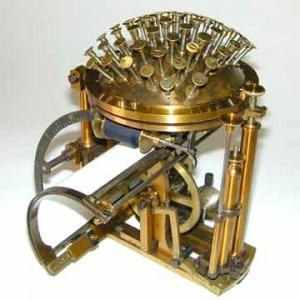
\includegraphics[width=5cm]{img/hansen.jpg}
\caption{Primjer pisaćeg stroja - Hansen writing ball (1870)}
\label{fig:hansen}
\end{figure}

Godine 1867. Cristopher Latham Sholes, uređivač novina iz Wisconsina, patentirao je svoj prvi pisaći stroj koji je razvio s prijateljima Carlos Glidden-om i Saumel W. Soule-om. Taj je stroj, kao i svi njegovi prethodnici, bio mehanički i zbog toga se već napisani znakovi nisu mogli samo tako izbrisati kao što to možemo danas na svojim računalima i mobitelima. Ukoliko je unio nešto krivo, korisnik je morao izvaditi papir i započeti iznova. Sholes je zbog toga želio osmisliti raspored znakova na tipkovnici koji bi korisniku omogućio da radi manje pogrešaka. Prijedlog je bio da razdvoji najčešće korištene parove slova (\emph{npr. "th" u engleskom jeziku}), tako da ne budu jedno pokraj drugoga, a i da korisnik naizmjence tipka s lijevom i desnom rukom. Da bi se to ostvarilo bilo je potrebno proučiti bigrame\footnote{Frekvencija pojavljivanja parova slova u pojedinom jeziku} za određeni jezik. Sholes se mučio nekoliko godina kako bi usavršio raspored dok konačno nije došao do onog kakav se i danas koristi.

\begin{figure}[htb]
\centering
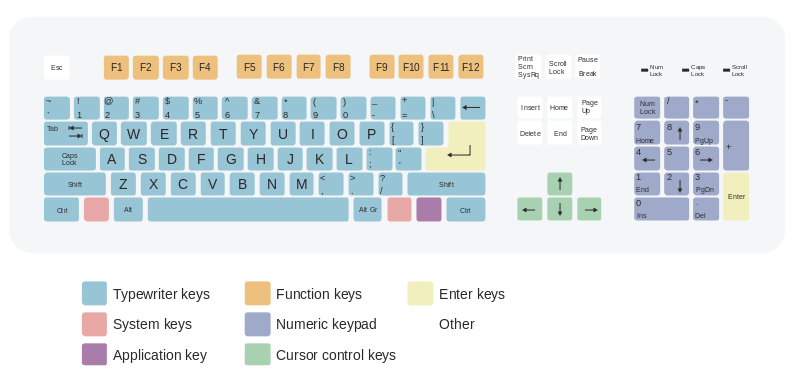
\includegraphics[width=12cm]{img/qwerty.png}
\caption{Standardni QWERTY raspored}
\label{fig:qwerty}
\end{figure}

\section{Tipkovnice danas}
Iako je QWERTY najpopularnija tipkovnica to ne znači da je i najučinkovitija. One se danas koristi zbog toga što su svi navikli na nju, lako je korisiti i teško je naučiti i preći na neku drugu. Postoji još mnogo različitih rasporeda i načina unošenja teksta koji su se eksperimentalno pokazali učinkovitijim od QWERTY. Navest ćemo neke od njih.


\chapter{Opis i rješenje problema}

\chapter{Ispitivanje rezultata}

\chapter{Zaključak}
Zaključak.

\bibliography{literatura}
\bibliographystyle{fer}

\begin{sazetak}
Sažetak na hrvatskom jeziku.

\kljucnerijeci{Ključne riječi, odvojene zarezima.}
\end{sazetak}

% TODO: Navedite naslov na engleskom jeziku.
\engtitle{Alternative Touchscreen Keyboard Based on Fitts Law}
\begin{abstract}
Abstract.	

\keywords{Keywords.}
\end{abstract}

\end{document}
